\documentclass[11pt,a4paper]{article}

\setlength{\textwidth}{165mm}
\setlength{\textheight}{240mm}
\setlength{\parindent}{0mm} % S{\aa} meget rykkes ind efter afsnit
\setlength{\parskip}{\parsep}
\setlength{\headheight}{0mm}
\setlength{\headsep}{0mm}
\setlength{\hoffset}{-2.5mm}
\setlength{\voffset}{0mm}
\setlength{\footskip}{15mm}
\setlength{\oddsidemargin}{0mm}
\setlength{\topmargin}{0mm}
\setlength{\evensidemargin}{0mm}

\usepackage{courier}
\usepackage{amsmath}
\usepackage[a4paper, hmargin={2.8cm, 2.8cm}, vmargin={2.5cm, 2.5cm}]{geometry}
\usepackage{eso-pic} % \AddToShipoutPicture
\usepackage{graphicx} % \includegraphics
\usepackage[english]{babel}
\usepackage[utf8]{inputenc}
\usepackage{amsfonts,amsmath,amssymb}
\usepackage[colorinlistoftodos]{todonotes}
\usepackage{gauss}
\usepackage{enumitem}
\usepackage{hyperref}
\usepackage{microtype}
\usepackage{listings} %code parsing
\lstset{language=bash} %java code
\newcommand{\code}[1]{\texttt{#1}}

\newlist{SubItemList}{itemize}{1}
\setlist[SubItemList]{label={$-$}}

\let\OldItem\item
\newcommand{\SubItemStart}[1]{%
    \let\item\SubItemEnd
    \begin{SubItemList}[resume]%
        \OldItem #1%
}
\newcommand{\SubItemMiddle}[1]{%
    \OldItem #1%
}
\newcommand{\SubItemEnd}[1]{%
    \end{SubItemList}%
    \let\item\OldItem
    \item #1%
}
\newcommand*{\SubItem}[1]{%
    \let\SubItem\SubItemMiddle%
    \SubItemStart{#1}%
}%

\newcommand{\BAR}{%
  \hspace{-\arraycolsep}%
  \strut\vrule % the `\vrule` is as high and deep as a strut
  \hspace{-\arraycolsep}%
}

\author{\Large{Sven Frenzel (\href{mailto:sven@frenzel.dk}{sven@frenzel.dk}) - 130793 - cdn769}\\
\Large{Mads Gram (\href{mailto:mgmadsgram@gmail.com}{mgmadsgram@gmail.com})  - 081293 - wtc324}\\
\Large{Thorkil Værge (\href{mailto:thorkilk@gmail.com}{thorkilk@gmail.com}) - 150287 - wng750} \\ \\
\Large{Instructor: Kasper Passov }}

\title{
\vspace{3cm}
\Large{First Partial Assignment - ProjDat}
}

\begin{document}

%% Change `ku-farve` to `nat-farve` to use SCIENCE's old colors or
%% `natbio-farve` to use SCIENCE's new colors and logo.
\AddToShipoutPicture*{\put(0,0){\includegraphics*[viewport=0 0 700 600]{include/natbio-farve}}}
\AddToShipoutPicture*{\put(0,602){\includegraphics*[viewport=0 600 700 1600]{include/natbio-farve}}}

%% Change `ku-en` to `nat-en` to use the `Faculty of Science` header
\AddToShipoutPicture*{\put(0,0){\includegraphics*{include/nat-en}}}

\clearpage\maketitle
\thispagestyle{empty}

\newpage
\tableofcontents{}
\thispagestyle{empty}


\newpage


\section{Project Definition}
\subsection{Overview of the Customer and the Project}
The Ph.D student Oleksandr Shturmov at the Department of Computer Science, University of Copenhagen has presented us with the project of mapping KU usernames to public OpenPGP keys and creating the guides for the students and writing the server backend and frontend to accomplish this. This system should be used by the students, the teaching assistants, and the teachers at the university to ensure the authenticity of the identity of the end-user, i.e., the student.
\subsection{Problem statement}
\subsubsection{Problem Domain}
At the University, many courses require the students to hand in assignments. In this modern era, this is done by electronic hand-ins over the World Web Web on the interconnected global network. It is essential to ensure that there can be no doubt of the identity of the student handing in the assignment because the teachers grade the students based on these electronic hand-ins. \\\\

This problem can be solved by a classic login system, where the user has a unique username and picks a password as a secret piece of information to avoid malicious parties to get access to user privileges. This system has already been implemented by the Norwegian company its Learning through the World Wide Web platform ``Absalon''.\\\\

Another option, which is the subject of this project, is to use asymmetric key encryption. In this system the user, i.e. the student, generates a key pair on his own computer. This keypair can be used for authentication and can also be used in other situations. The authenticity of the key pair can be further validated by peer-to-peer authentication through the signing of other peoples' keys.\\\\

The students at the University of Copenhagen all have a unique username in the form of a ``KU Username''. If this username is mapped to a public key and the student holds the equivalent private key, then the authentication of an electronic hand-in has the same degree of trusted authenticity as that of the key pair. \\\\

We can use the KU login in order to establish this mapping and this mapping can be further authenticated by the above-mentioned peer-to-peer key signing although this latter authentication is not necessary for the system to work. I.e., support for peer-to-peer signing in this project is nice-to-have, not need-to-have. As a way to establish this mapping, the KU login is used as a trusted source of linking an identity to a public key. The role, if any, of peer-to-peer signing or key signing by teachers has not yet been established.


\subsubsection{Scenarios}
\begin{itemize}
\item A student has just started on the course ``Maskinarkitektur'' (Processor Design). He learns that he has to hand in the assignment by signing it with an OpenPGP key. He must then generate his own key pair using a designated program like ``GPG4Win'' or through a webservice developed as a part of this project and hosted by KU. After the key pair has been generated, the student uploads his public key to a server and the server then stores the KU Username and the public key.
\item When the student hands in his assignment, he signs it with his newly generated private key. And the signature is then uploaded along with the assignment. A teacher is grading the assignments that has been handed in on the course ``Maskinarkitektur''. Before he grades them, he needs to check the validity of the identity of the student. This check can either be done automatically by software that interfaces with the system developed as part of this project or manually by the teacher.
\item All teachers have their OpenPGP-keys on the service and sign all feedback. These public keys must be available for the students.
\end{itemize}

\subsubsection{Solution Domain}

To solve the aforementioned scenarios we have drafted a solution, which employs a key-server that will act as an authority. It will contain OpenPGP-keys for all users of the system. To validate the users it will use their KU e-mail, which is created by other parts of KU, and thereby validated. A mapping of these two components will be created as core database of the system.\\

As part of the system, a web-server will be established, which will facilitate the replacement of OpenPGP-keys in the case of loss of a users private key. This web-server also serves as point-of-contact for the initial creation of users. The aforementioned validation will be facilitated by an integrated e-mail server. \\

Upon creation of a user, a unique link, containing all necessary info, will be generated and served to the users KU e-mail. When this link is accessed by the user, they are offered to upload their own OpenPGP-keys, generated in dedicated software like "PGP4Win" or to create a new OpenPGP-key in the browser by using a HTML5/JavaScript based OpenPGP-key generator.\\

The replacement of the key will be processed in the same way, as the initial upload of a key, with the one exception, that the user manually has to request, that a new upload link will be sent to their KU e-mail.

% :I

\subsubsection{Functional Requirements}
\begin{itemize}
\item The system must map a KU Username to a OpenPGP public key.
\item Users must be able to upload their own public key to the service.
\item If a user loses his private key, a method for replacing the public key must exist.
\item The initial registration of a key, and the replacement of a key, is authenticated through the KU email system.
\item Lookups in this table must be possible for the relevant university staff. An API will be defined and implemented for this.
\item The KU usernames must not be accessible for outsiders.
\item A guide for creating key pairs needs to be available on the website, possibly as shell script. This guide should explain how to derive an SSH key from an OpenPGP key.
\end{itemize}
\subsubsection{Nonfunctional Requirements}
\begin{itemize}
\item The backend should be written in golang.
\item The frontend should be Javascript and/or HTML5, which ever is safest and most easy to use.
\item The system should be browser independent.
\item The system must be compliant with all standards and regulations imposed by the Government of Denmark and the University of Copenhagen. These regulations will be within privacy and will regard the KU usernames that are part of the system.
\item The customer has decreed, that the software be licensed under a MIT-like license, which will be provided by the customer.
\end{itemize}
\subsubsection{Target Environment}
\begin{itemize}
\item The frontend must work on the newest editions of all mainstream browsers -- Internet Explorer, Firefox, Chrome, Safari.
\item The backend software must be able to run on the most popular Unix-like systems.
\end{itemize}
\subsubsection{Delivarables and Deadlines}\label{sec:deadlines}
\begin{itemize}
\item A preliminary version must be ready for testing and security auditing by mid May.
\item The whole project must be done by June 3$^{rd}$, 2015.
\item A list of documents to be delivered together with the software can be read in Section \ref{sec:deliverables}
\end{itemize}
\subsection{Initial Software Project Management Plan}
\subsubsection{Work Breakdown}
The following tasks have been identified. The list is subject to change.
\begin{itemize}
\item Acquire VPS
\item Initial set-up of VPS
\SubItem Install Go compiler
\SubItem Install SQLite or postgresql
\SubItem Create startup script for server to run appropriate programs.
\item Use golang to connect to database
\item Determine exact method for teachers to fetch data from DB API
\item Front-end view containing a form for first-time upload of OpenPGP key
\item Front-end view which enables replacement of key
\item Mail server to send links for students to upload OpenPGP key
\SubItem System that creates signed single-use links for key upload
\end{itemize}
\subsubsection{Roles \& Responsibilities}
This group consists of Mads Gram, Sven Frenzel, and Thorkil Værge. The roles and responsibilities have not yet been delegated. So instead, we choose to describe our individual skill set.
\begin{itemize}
\item Mads Gram: Can code Javascript for front-end, some knowledge of MVC architecture, SQL and general DB knowledge
\item Sven Frenzel: Linux server administration, basic network administration. Has experience with HTML and CSS and is a proficient bash scripter.
\item Thorkil Værge: Some experience in project management of website development, SQL experience from DB course, some front-end experience with HTML and CSS. Theoretical knowledge of hashes and cryptography and practical knowledge of internet security.
\end{itemize}
\subsubsection{Project Schedule}
We have chosen to divide the project schedule into phases. In the spirit of agile development, the following list should be viewed as an iterative process and something that will overlap a lot. Some of these tasks could also be given a deadline under Section \ref{sec:deadlines}.
\begin{itemize}
\item Defining the project -- the introductory phase where we iteratively align our expectations for the project with the customer's expectations.
\item Learning Go -- this can be done through some very basic Go tutorials but will probably mainly be achieved by reading up on how a Go server is built and connects to a server as well as implementing this setup.
\item Obtaining additional required skill set: some front-end development in HTML5 or Javascript.
\item Setting up the server with required programs, including e.g. Go compiler and SQL server.
\item Programming the server and its SQL interaction in Go.
\item Programming the front-end.
\item Setting up email server to talk to Go on our VPS.
\item Presenting results to customer for feedback.
\item Testing the programmed logic.
\end{itemize}
\subsubsection{Budget and Resources}
The following resources are required for the project and will be provided by the customer.
\begin{itemize}
\item VPS or dedicated server.
\item access to a mail server (Oleks researches).
\item Subdomain on customer's server to host the PGP registration website.
\item SSL certificate to defeat man-in-the-middle attack where an attacker sends a fake public PGP key to the server.
\item time resources: As of yet unknown but we expect that large parts of the programming can be solved at intensive work weekends.
\end{itemize}
\subsubsection{Description of Risks}
\begin{itemize}
\item There is a risk that learning Go will be too complex a task for us to master in time. To mitigate this risk, a deadline for some basic server functionality, using Go, should be made. We set a deadline for May 1$^{st}$ for getting the VPS to connect to the database through Go. This task requires basic Go knowledge and will test our basic Go abilities.
\item During the security audit, serious vulnerabilities could necessitate major restructuring of the code base.
\end{itemize}
\newpage
\subsection{Initial software architecture}
See Figure \ref{fig:ISA} \\\\

\begin{figure}[h!]
\centering
%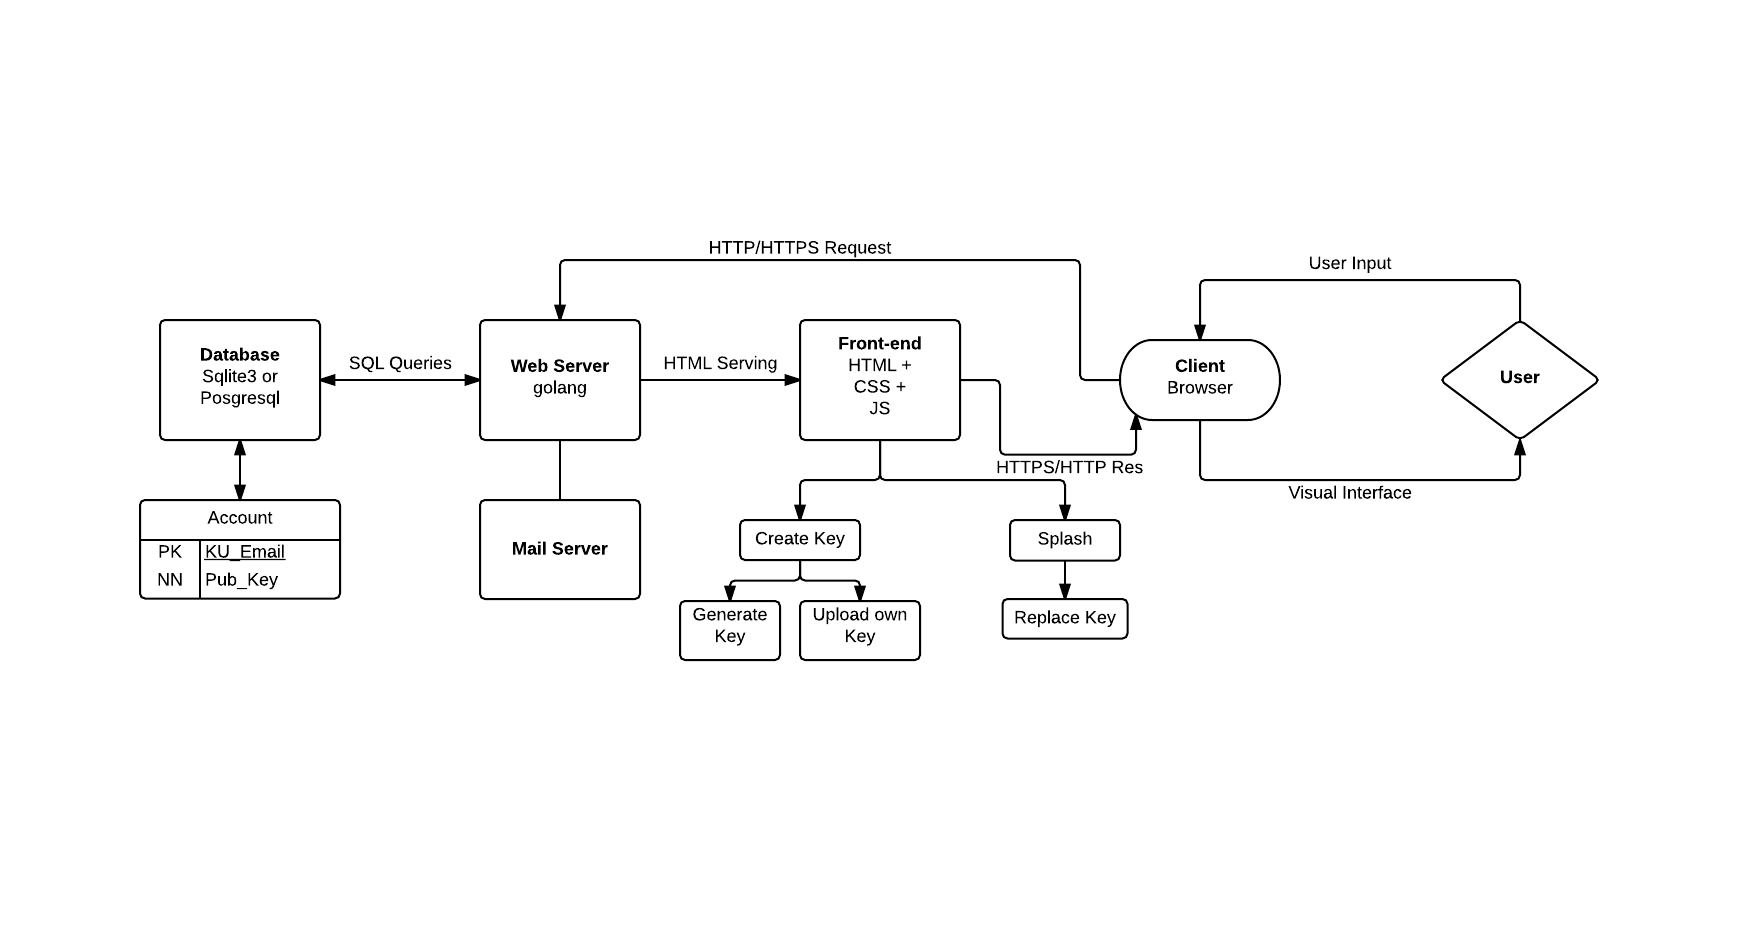
\includegraphics[width=1.1\textwidth]{pictures/pksu_isa_centered}
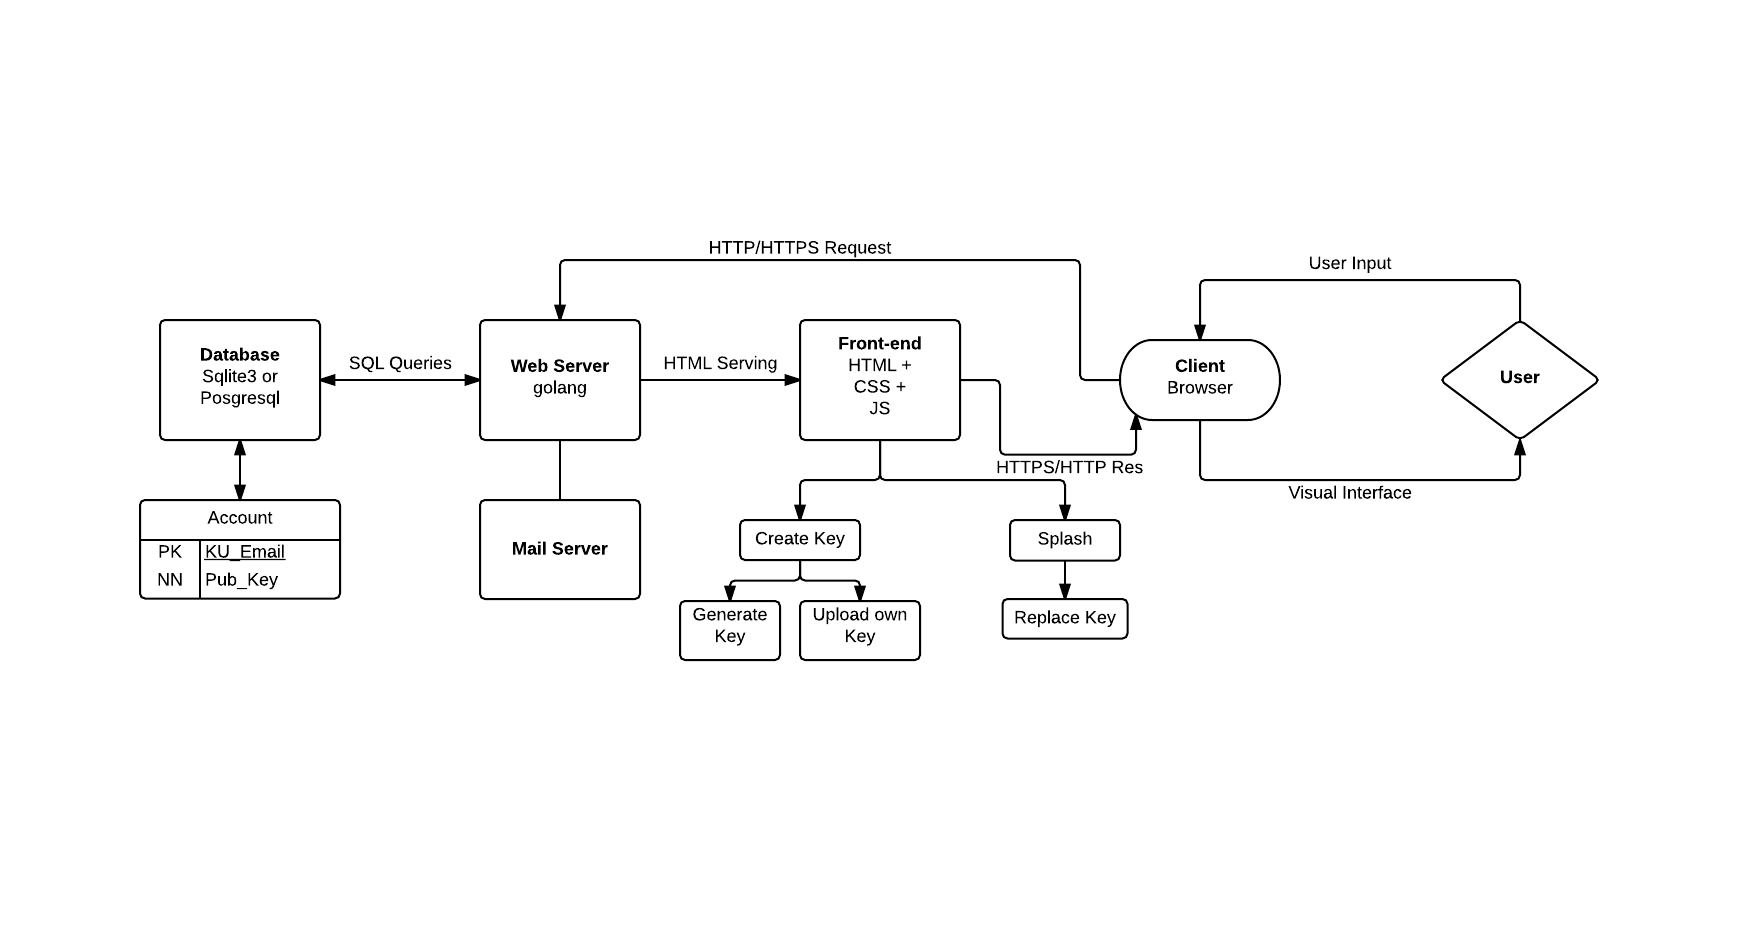
\includegraphics[width=1.1\textwidth]{pictures/pksu_isa_centered}
\caption{Initial software architecture of the project. Our project includes coding the database, web server, and front-end.}
\label{fig:ISA}
\end{figure}

\subsection{Project Agreement Definition}
The purpose of the Project Agreement Definition (PAD) is to outline the Project Agreement (PA) which is a contract that we, the developers, and the customer agree upon. A contract defining the duration, cost, deliverables, and minimum requirements for the project should be defined. The sections below are drafts of the contents of the PA which is yet to be fully defined and has \textbf{not} been approved of the customer. The next meeting should have the PA on the agenda.
\subsubsection{List of Deliverable Documents}\label{sec:deliverables}
\begin{itemize}
\item Source code of the project.
\item Technical documentation of the developed system.
\item Non-technical report describing the system in layman terms.
\item Scripts and/or guides for set-up of the developed server software.
\SubItem A report documenting set-up of all dependencies for the developed system, including, but not limited to, a log of all commands used to set-up the development environment.
\item Working server running compiled software.
\item Report of security audit.
\end{itemize}
\subsubsection{Criteria for Demonstrations of Functional Requirement}
All aspects of the basic functionality must be tested thoroughly. This includes tests of uploading of public keys, replacement of private keys, administrator access to the private keys and more.

\subsubsection{Test suite:}

We will develop a test suite along with the system. This will be used internally to ensure that the logic is sound and that all functions run correctly. Furthermore it will also serve as a way to monitor the progress of the system.\\
Since multiple developers will be working on the code base, it is a genuine concern that changing the code can course problems throughout the code base. In that case, the test suite will check that such problems are not overlooked since the test suite will highlight the problems.\\
In the end, the test suite will be extended and be used as a validation of the system. The test suite will serve as the primary validation of the functional requirements. \\\\
In our specific case, some preliminary test will focus on correct execution of the individual cases. Then as the project evolves and becomes more interwoven, tests will be written also check the more complex functionality.

\subsubsection{Criteria for Demonstrations of Non-functional Requirements}
All aspects of the website should be tested and look uniform on all four standard web browsers.
Security-wise, the customer has expressed certain requirements. It must not be possible for non-approved persons to access the list of KU usernames since the university has not published this list and this then would consititute a loss of privacy for the students. It is however acceptable that the usernames are stored in plaintext on the server.
\subsection{(e)}
\section{System definition - FACTOR}
\textbf{F:} Return a cryptographic identifying value paired with a KU-ID. \\
\textbf{A:} Verification of the authenticity  of a person. \\
\textbf{C:} The current system for handing in assignments is hugely unpopular and a method for verifying the sender of an assignment in a new, yet to be developed, system is needed.\\
\textbf{T:} Servers with a UNIX-like OS for back-end, modern browsers for front-end. \\
\textbf{O:} Students and staff at KU. \\
\textbf{R:} Identity lookup tool.\\



\newpage
\section{Exercises from Weekly Assignments}

\subsection{OOSE 1-6:}
Specify which of these statements are functional requirements and which are
nonfunctional requirements\\\\
- “The TicketDistributor must enable a traveler to buy weekly passes.”\\
This first requirement is a \textbf{functional} requirement, since it is an essential function of the system.\\\\
- “The TicketDistributor must be written in Java.”\\
This is a \textbf{non functional} requirement.\\\\
- “The TicketDistributor must be easy to use.”\\
This is a \textbf{nonfunctional} requirement, an reason for this is that it can't be objectively answered. It is not possible too be simply evaluated as easy or hard to use.\\\\
- “The TicketDistributor must always be available.”\\
This is a \textbf{functional} requirement. \\\\
- “The TicketDistributor must provide a phone number to call when it fails.” \\
This is a \textbf{functional} requirement, since it describes a concrete function of the system.\\


\subsection{OOSE 1-8:}
In the following description, explain when the term account is used as an application domain concept and when as a solution domain concept.\\\\
In this specific example from the given text, we see the Application Domain is the issue of users not always being online. Which limits the customer to access to their account.\\
In this specific example from the given text, we see the Solution Domain, as the proposal of giving the user the data from the last connected session.\\
\newpage
\subsection{OOSE 2-6:}

\begin{figure}[h!]
    \centering
    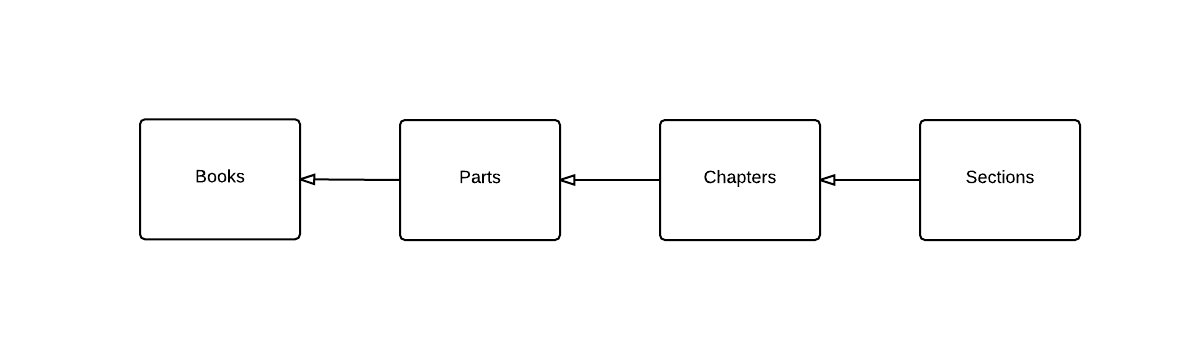
\includegraphics[width=1.1\textwidth]{pictures/oose2_6}
    \label{fig:OOSE26}
\end{figure}

\subsection{OOSE 2-7:}
\begin{figure}[h!]
    \centering
    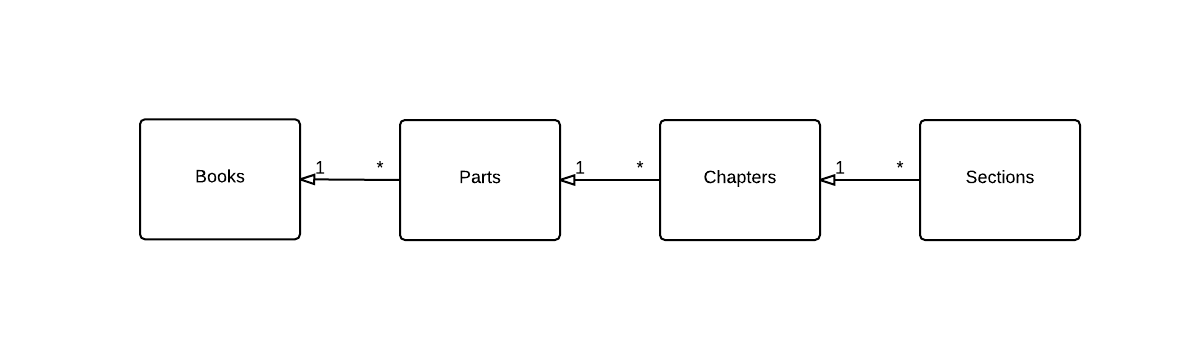
\includegraphics[width=1.1\textwidth]{pictures/oose2_7}

    \label{fig:OOSE27}
\end{figure}


\newpage
\subsection{OOSE 2-9:}

\begin{figure}[h!]
    \centering
    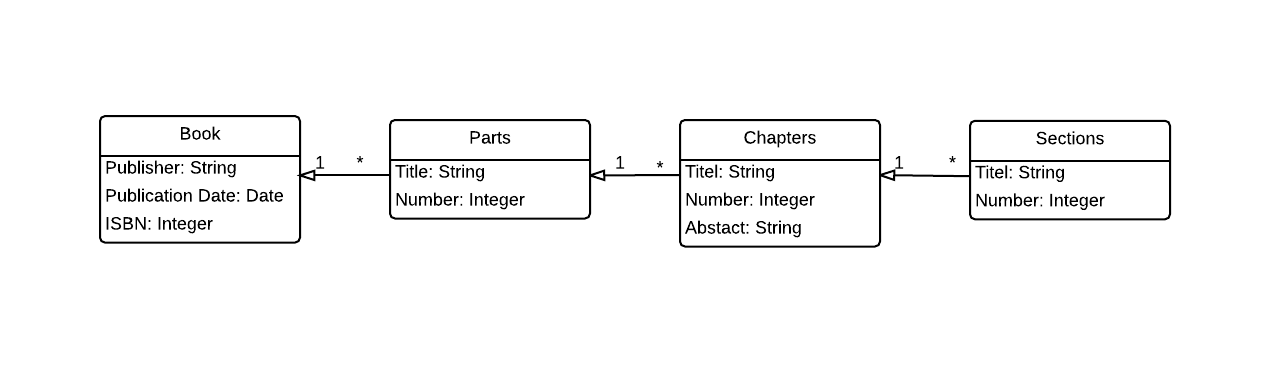
\includegraphics[width=1.1\textwidth]{pictures/oose2_9}

    \label{fig:OOSE29}
\end{figure}

\subsection{OOSE 2-10:}

\begin{figure}[h!]
    \centering
    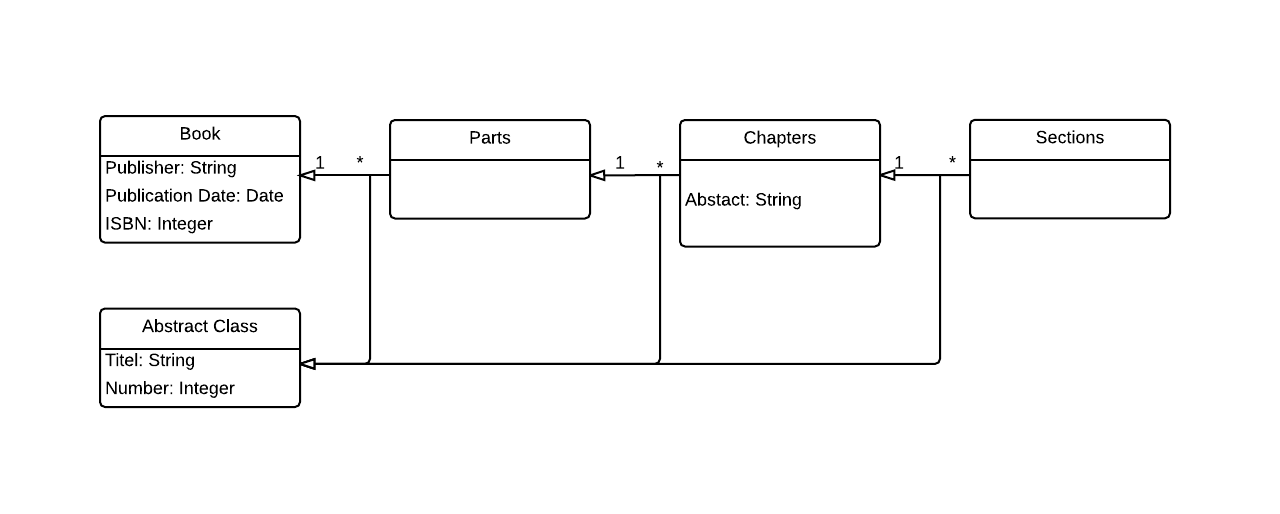
\includegraphics[width=1.1\textwidth]{pictures/oose2_10}

    \label{fig:OOSE210}
\end{figure}

\newpage
\subsection{OOSE 7-1:}

\begin{figure}[h!]
    \centering
    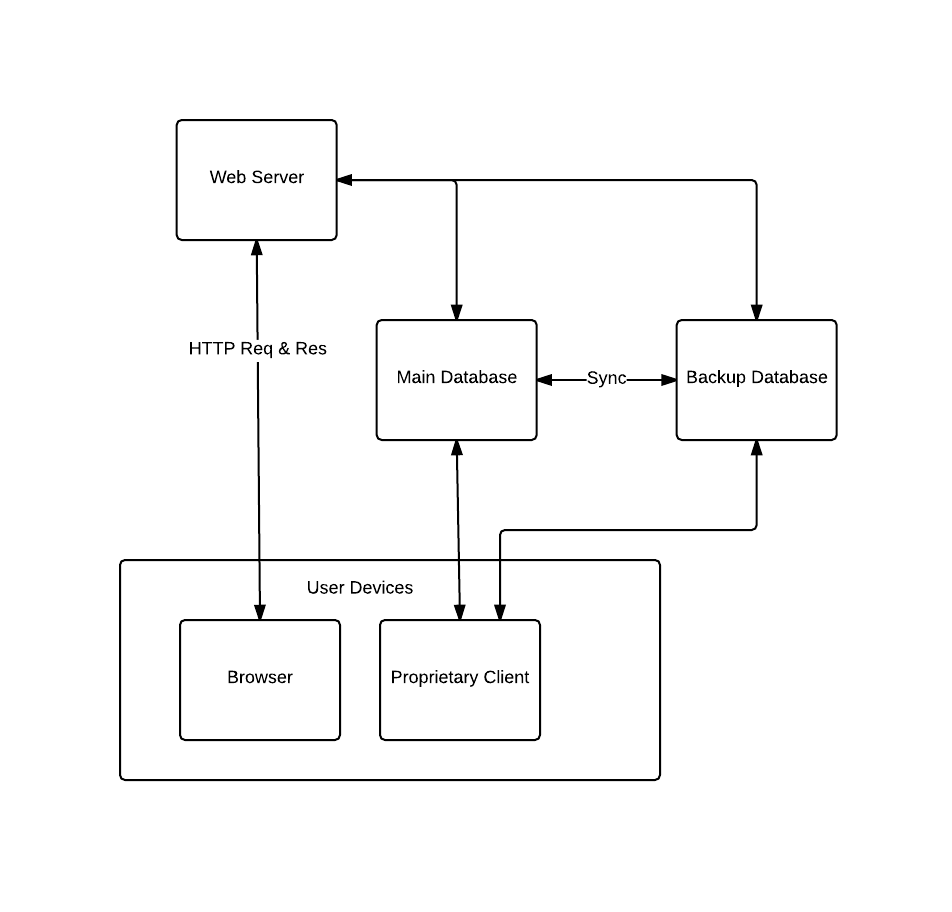
\includegraphics[width=1.1\textwidth]{pictures/oose7_1}
    \label{fig:OOSE71}
\end{figure}

\newpage
\section{Appendix}
\subsection{Minutes from March 16th 2015}
\begin{itemize}
\item Ønsker: identificer studerende ved aflevering vha gpg-nøgle
\item Ønsker: grube med gpg-nøgle og ku-mail knyttet sammen (da der stoles på at den studerende har adgang til sin email)
\item Autentificering sker igennem unikke links til ku-mail (for at lægge gpg-nøgle op).
\SubItem 2 muligheder: copy/paste gpg-nøgle eller generer gpg-nøglepar direkte i browseren.
\item DIKU leverer ssl-certifikat.
\item Hvorfor ikke bruge eksisterende?
\item Public index j/n?
\item modtager ukrypteret nøgle og bruger den til at verificere indholdet - bagefter checkes hashet pubkey mod databasen.
\item Arbejdsbelastning: 10 timer per person per uger
\item database: (\underline{ku-nummerplade},hash(pubkey))
\end{itemize}
\subsubsection{Krav:}
\begin{itemize}
\item registrering gennem webformular og/eller kommandelinje
\item skal kunne genregistrering
\item anmodning kodkendes igennem ku-email
\item kunne vælge om den offentlige nøgle offentliggøres
\SubItem private by default
\item private API: få offentlig nøgle og returner brugernavn (kun adgang til DIKU-ansatte)
\item Sprog
\SubItem Backend: golang + sql
\SubItem frontend: html5 + js
\end{itemize}

næste møde:
2015-03-22 kl 11-16

\subsection{Minutes from March 22nd 2015}
The meeting was held to align the expectations of the client and the developers in regards to the systems capabilities and design.

\begin{itemize}
\item Oleks undersøger interface hvilke tilgangsmuligheder, der ønskes til databasen.
\item Kun lukket API, intet offentligt look-up. Der gemmes pupkey og abc123 (ku-brugernavn).
\item key-server i stil med MIT-keyserver er nice-to-have. Man bliver kun listet her, hvis man eksplicit ønsker dette.
\item Den studerende uploader en fil til afleveringssystemet (uden anden information). Afleveringssystemet anmoder om par af PubKey \& KU-ID og undersøger om filen er signeret af denne nøgle. Hvis ikke, så anmodes næste par indtil det korrekte par er fundet. Dette returneres til underviser.
\item Beta klar til start/midt maj.
\item Oleks gives a license (MIT-like)
\item ISA-diagram
\SubItem Fjern Admin-login fra (der er sshd-adgang til serveren anyways.)
\SubItem Front-end til client, er response og ikke request
\SubItem User guide /shell script ved "Create key"
\item Oleks anmoder om at der sendes en dagsorden 24 timer før fremtidige møder
\item Thorkil foreslår at møder optages auditivt.
\end{itemize}

Næste møde er 29/30 marts 2015.


\end{document}
